% !TEX root =  ../main_manuscript.tex 
\section{Introduction}
Patients with low- and very low-risk screening-detected localized prostate cancer (PCa) are usually advised active surveillance (AS) instead of immediate radical treatment \citep{briganti2018active}. In AS, PCa progression is routinely monitored via prostate-specific antigen (PSA), digital rectal examination, and the Gleason score from repeat prostate biopsies. Since Gleason score is the strongest indicator of cancer-related outcomes, patients are commonly advised curative treatment when Gleason~$\geq$~7 (GS7) is detected \citep{bul2013active}.

Biopsies are conducted periodically, and hence GS7 is always detected with a time delay. The smaller this delay, the larger is the window of opportunity for curative treatment. For timely detection of GS7, many AS programs use fixed biopsy schedules (e.g., annual or biennial biopsies) for all patients \citep{nieboer2018active,loeb2014heterogeneity}. However, many AS patients do not require any biopsy in the first ten years of follow-up (see PRIAS and John's Hopkins AS cohorts in Figure~\ref{fig:npmle_plot}). Biopsies are also invasive, painful and prone to medical complications. Biopsy burden combined with patient non-compliance \citep{bokhorst2015compliance} to frequent biopsies, has raised concerns regarding the optimal biopsy schedule \citep{inoue2018comparative, bratt2013study}.

\begin{figure}[!htb]
\centerline{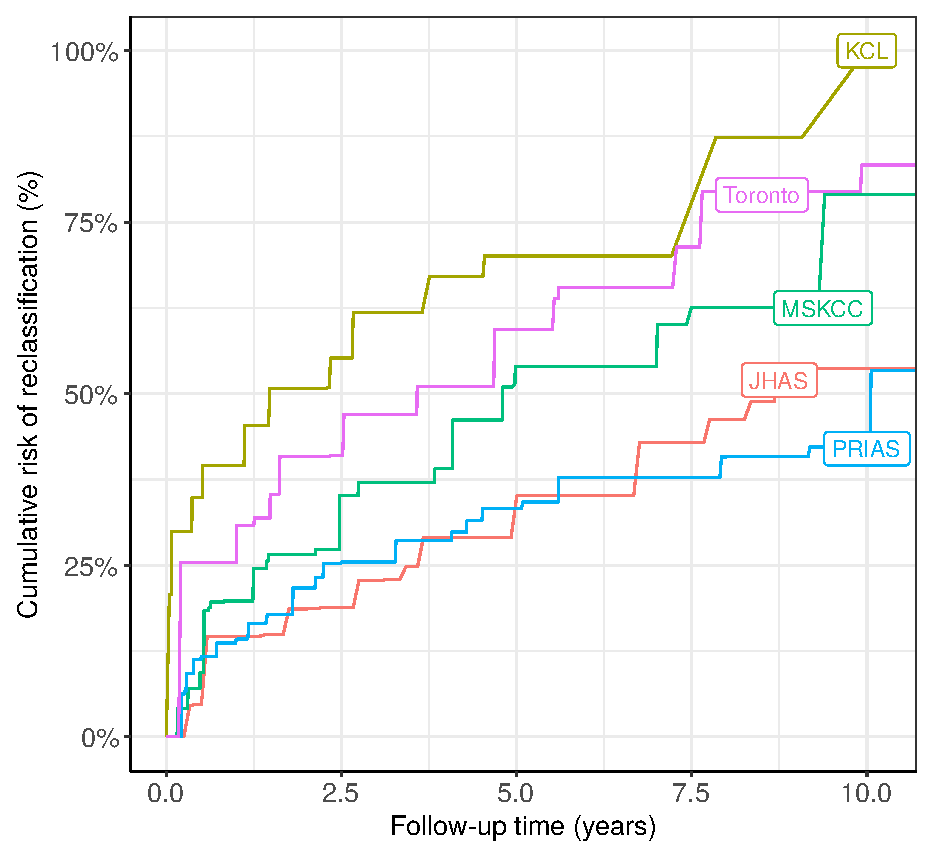
\includegraphics[width=\columnwidth]{images/npmle_plot.eps}}
\caption{\textbf{Estimated cumulative risk of having Gleason~$\geq$~7 (GS7)} in the world's largest AS cohort PRIAS, and five of the largest AS cohorts part of the GAP3 database \citep{gap3_2018}. Abbreviations are \textit{JHAS}: Johns Hopkins Active Surveillance, \textit{PRIAS}: Prostate Cancer International Active Surveillance, \textit{Toronto}: University of Toronto Active Surveillance, \textit{MSKCC}: Memorial Sloan Kettering Cancer Center Active Surveillance, \textit{KCL}: King's College London Active Surveillance. In the world's largest AS cohort PRIAS and in JHAS, roughly 50\% of patients do not obtain GS7 in the first ten years. That is, ideally no biopsies should be prescribed to 50\% of the patients in first ten years of AS.}
\label{fig:npmle_plot}
\end{figure}

A simple alternative to frequent biopsies is infrequent biopsies. However, studies suggest not reducing biopsy frequency beyond 24 months, to have a sufficient window of opportunity for curative treatment \citep{inoue2018comparative,de2017estimating}. Although, biopsy every 24 months still leads to five unnecessary biopsies over ten years for 50\% patients (Figure~\ref{fig:npmle_plot}). A promising alternative to fixed biopsies is biopsies based on personalized risk of GS7. For example, among the two patients shown in Figure~\ref{fig:riskBasedExample}, patient B is a more suitable candidate for biopsy than patient A, because his risk of GS7 is much higher. %Simulation studies have shown that personalized schedules may better balance the number of biopsies per detected GS7 than fixed schedules \citep{tomer2019}. 

\begin{figure}[!htb]
\centerline{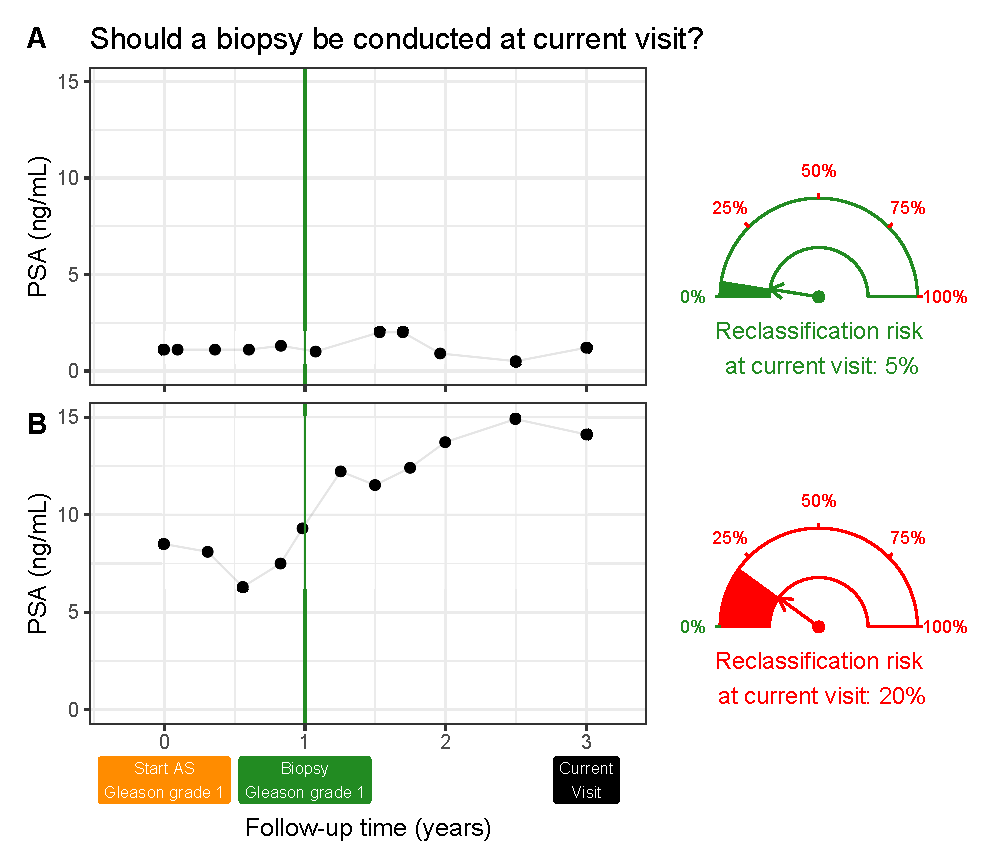
\includegraphics[width=\columnwidth]{images/riskBasedExample.eps}}
\caption{\textbf{Motivation for personalized risk-based decisions of biopsy}: Patient A and B had their latest biopsy at year one of follow-up. Patient A's prostate-specific antigen profile remained stable until the current visit time at year three, whereas patient B's profile has shown a rise. Consequently, patient B's estimated cumulative risk of GS7 at year three is higher than that of patient A, making patient B a more suitable candidate for biopsy than Patient A. Risk estimates in this figure are only illustrative.}
\label{fig:riskBasedExample}
\end{figure}

The first challenge in developing risk-based schedules is consolidating observed patient data (e.g., PSA, previous biopsy results) into GS7 risk estimates. Previousy, studies have utilized latest value of PSA to predict the Gleason score \citep{partin1993use,makarov2007updated}. However, in AS the entire trajectory of PSA of a patient is available. To accomodate such longitudinal PSA data, a suitable model is joint model for time-to-event and longitudinal data \citep{tomer2019,coley2017prediction,rizopoulos2012joint}. A subsequent challenge is to translate risk estimates for GS7 into clinical decisions is challenging. For example, a 10\% risk can be perceived as high/low depending upon the patient's age. Patients may also weigh the risk of GS7 with the potential consequences of another biopsy. Two relevant consequences are the timing and total number of biopsies (burden), and the time delay in the detection of GS7 (smaller is better). These consequences vary between the patients, and also over the follow-up period for the same patient.

The goal of this work was to assist patients and doctors in making better decisions of biopsies than fixed and frequent biopsies. We intended to achieve this by providing the patients risk based personalized schedules of biopsies, and to allow them to compare the consequences of each schedule before making a decision. To this end, we took three steps. First we fitted a prediction (joint) model to the world's largest AS dataset, PRIAS \citep{bul2013active}. We then externally validated the model predictions in five largest AS cohorts that are part of the GAP3 database. Lastly, we utilized the personalized GS7 risk predictions to calculate the timing and total number of biopsies, and the time delay in the detection of GS7 for risk-based and fixed biopsy schedules.